\chapter{Usage of {\it Elib}} \label{chap:usage}
  This chapter is aimed at a programmer who wants to start working with an e-Puck using {\it Elib}. 
  {\it Elib} offers a lot of tools, which make e-Puck programming easier. 
  The tools are useless without a proper use. This chapter introduces guidelines and numerous
  examples how to use {\it Elib} and avoid problems.
  
  On thirteen samples from {\it TestElib} project we present {\it Elib} and e-Puck's properties.
  The samples are written in $C\#$ and are densely commented.
  We suggest a programmer, who wants to program his e-Puck, to start with one of the examples
  from {\it TestElib} project and modify it according his needs.
  {\it Elib} is built robustly and improper use does not destabilise the operating system.

  Let us note that this chapter describes the use of {\it Elib} and its tools,
  but does not explain basic .Net or $C\#$ features. The basic knowledge of .Net and $C\#$ language is required
  for understanding {\it Elib} examples. On the other hand .Net $delegates$, an $EventWaitHandle$ class and usage of lambda functions in $C\#$
  are shortly introduced. A great part of this chapter is devoted to $IAsyncResult$ interface and its
  usage in {\it Elib}.

  {\it Elib} library requires .Net 2.0 on Windows and requires Mono 2.0 %todo verze mona?
  and higher on Linux.
  As an example of an application, which uses {\it Elib}, we present {\it Elib Joystick} at the end of this chapter.
  {\it Elib Joystick} is a graphical application, which uses Windows Presentation Foundation. It requires .Net 3.5 or higher
  and is not portable to Linux.
  {\it Elib} can control every actuator and get every sensor value with {\it BTCom}'s version 1.1.3 on e-Puck. 
  {\it BTCom} is a simple program running on e-Puck. It receives commands from {\it Elib}, performs the relevant actions
  and sends confirmation answer back. If we ask for a sensor value, the value is added to the confirmation message.

  The source codes are deployed using a solution of Microsoft Visual Studio 2008 (MSVS) for Windows 
  and MonoDevelop solution for Linux.
  If you use higher version of MSVS or MonoDevelop, then the solution can be easily upgraded.	

  The contents of this chapter is divided into 6 sections.
  The first section is devoted to advanced .Net techniques, which are used in {\it Elib}.
  The Section ~\ref{sec:interfaces} shortly introduces features of each {\it Elib's} interfaces and 
  it presents e-Puck's sensors and actuators.
  The next section goes through samples of implemented behaviours 
  from~{\it TestElib} project and explains the crucial part of the examples.
  The Section ~\ref{sec:et} presents the {\it Elib Tools} console application, 
  which is useful during developing a program for e-Puck.
  Finally the last section sums up the most important guidelines for {\it Elib} library.
  It also shortly points out, which algorithms and applications can profit most
  from {\it Elib} design and which applications bring problems.
  
\section{Advanced .Net techniques} \label{sec:net}
  {\it Elib} interface requires knowledge of $delegates$. Lambda functions and $EventWaitHandle$ class
  are used in {\it TestElib's} samples and asynchronous programming is much more comfortable with them.
  If you are familiar with terms above, their usage in {\it Elib} will be described in~ Section~\ref{sec:iabehaviors}.
  This section describes them in general.

  Delegates are .Net wrappers for functions. Every .Net language is strongly typed and even functions are typed in .Net.
  A delegate has two meanings in .Net. The first meaning is the placeholder type for functions of given type. 
  See the $C\#$ implementation in~Figure~\ref{deleg}. The placeholder type has name $OkfActuators$.
  The second meaning is the placeholder itself. In the sample code below the placeholder is called $a$.

  Delegate variable can contain functions, which exactly match delegate definition. In the case of $OkfActuators$ 
  delegate from~Figure~\ref{deleg} the function must return
  $void$ and it must have one argument of type object. All classes in $C\#$ are inherited from $Object$ class, 
  therefore every object can be passed to this delegate. 
  Object class contains method $ToString()$ and therefore the number as well as the string are printed.  
  Delegate function can contain more functions. On the other hand this feature is not used in {\it Elib}, 
  because it reduces readability of the code.
  

\begin{figure}[!hbp]
\begin{lstlisting}[language=cs]
// Delegate definition in some class e.g Program
delegate void OkfActuators(object data);
void Example(){
  int i=8;
  //declaration of delegate variable and initialization with lambda function
  OkfActuators a = new OkfActuators((sth) => { Console.WriteLine("Lambda f{0},{1}",sth,i); });
  //second function is added to delegate
  a += new OkfActuators(suitableFunction);
  //invocation of 2 functions with string parameter
  a("Hurray!");
  //third function is added to delegate
  ExampleClass c=new ExampleClass();
  a+= new OkfActuators(c.suitableMethod);
  //invocation 3 functions with int parameter.
  a(-333);
}
private static void suitableFunction(object sth) { 
  Console.WriteLine("suitable Function {0}",sth);
}
class ExampleClass{
  public void suitableMethod(object sth) { 	
          Console.WriteLine("suitable method {0}",sth);	
  }
}
/\end{lstlisting}
\caption{Definition of a delegate} \label{deleg}

%output
\begin{verbatim}
Lambda fHurray!,8
suitable Function Hurray!
Lambda f-333,8
suitable Function -333
suitable method -333
\end{verbatim}
\end{figure}
  The console output of $Example()$ function shows, that the functions are called in the order, in
  which the functions were added to the delegate variable. 
  The functions have void returning value, because there is no chance how to access
  the returning value from the first function. Delegates allow the last function to return its value, 
  but it is considered a bad manner, because
  another function added to delegate can overwrite the returning value of the delegate call.

  Let us focus on the function, which is used in the $OkfActuators$ declaration. The function 
  was defined and declared in place. Functions defined in place are called lambda functions 
  and have several advantages. 
  They can omit types of arguments, because they are inferred from delegate definitions. Lambda functions
  can also directly use variables from the scope of its declaration. 
  The lambda function printed $8$ in the enclosed output above,
  although we have not passed it as an argument to the delegate.

  %todo I have to PASTE TEXT DESCRIBING EventWaitHandle
  \begin{definition}[$EventWaitHandle$]
  %citace od Preklad „Threading in C#“ od Josepha Albahari
  %sekce 2.5.1
  The $EventWaitHandle$ class 
  \end{definition}
  $EventWaitHandler$ class is not tricky itself, but sometimes it is used in multi thread programming, which is usually complicated.
  An instance of the class is used to synchronise two threads. It is usually used to signal from one thread to another, 
  that some work has been done. In {\it Elib} there are used two methods per~$EventWaitHandle$ instance.
  Let us suppose we have a thread $A$ running. Let $B$ be the thread, which should perform a long task. 
  The thread $A$ wants after a while to wait until the work of $B$ is finished.
  Before the job $B$ finishes. $A$ creates $EventWaitHandle$ $e$ with parameters $false$ and $ManualReset$. 
  $False$ parameter sets $e$ to a blocking state. In the blocking state all threads, which have called method $e.WaitOne$, 
  are synchronously blocked in $WaitOne$ method. $ManualReset$ means that the state of $EventWaitHandle$ 
  can be changed only by its methods and $EventWaitHandle$ does not perform any action itself.
  Let us return back to threads $A$ and $B$. $A$ creates an instance $e$ of $EventWaitHandle$ with mentioned parameters, 
  passes $e$ to the second thread. 
  Finally $A$ calls $WaitOne$ and blocks on this call.
  $B$ thread works and after the job is done, it just invokes $Set$ method on $e$. 
  $Set$ method releases all threads, which are blocked in $WaitOne$ method.
  Run the code from the snippet ~\ref{ewh} to understand it.

          
\begin{figure}[!hbp]
\begin{lstlisting}[language=cs]
static EventWaitHandle e = null;
static void Athread() {
  Thread t = new Thread(Bthread);
  e = new EventWaitHandle(false, EventResetMode.ManualReset);
  t.Start();
  e.WaitOne();
  Console.WriteLine("Finally someone press the button!!!");
}
static void Bthread() {
  //simulate the work      
  Console.Readline();
  e.Set();
}
\end{lstlisting}
\caption{Definition of a delegate} \label{ewh}
\end{figure}

   $EventWaitHandle$ is used in the function $endBehaviour$ described in Section ~\ref{sec:iabehaviors} 
   used in behaviour implementation.
   Lambda functions can be seen for example in $ConsoleTestSensorsTimeout$ function, which presents all sensors from e-Puck.
   Delegates are used in every command invocation to specify types of callback functions.
   Callback functions are functions, which are called after finishing an operation. 
  
\section{Explore {\it Elib} through examples} \label{sec:interfaces}
  There are three public classes in {\it Elib}. $Sercom$, $Epuck$ and $Stamp$.
  $Stamp$ is for time measurement. $Sercom$ and $Epuck$ are classes, where all the algorithms are located.
  $Epuck$ class uses $Sercom$ internally.
  Let us focus only on $Epuck's$ class, because $Epuck$'s basic interface is a specialisation of~$Sercom$'s
  interface for version 1.1.3 of {\it BTCom}.
  For more information about interfaces and implementation of $Sercom$ and $Epuck$ see Section ~\ref{chap:elib}.

  $Epuck$ class itself has two interfaces. Let us name them the basic interface and $IAsyncResult$ interface.
  $IAsyncResult$ interface is used widely through .Net. We will introduce it in the examples from {\it TestElib} project.
  All examples from this section come from {\it TestElib} project. We suggest reading this chapter with {\it TestElib} project opened
  and explore the samples from {\it TestElib} in detail.


  %todo in the paragraph below I HAVE TO ADD REFERENCES!!
  The examples are listed from the simplest to the more complex. 
  First function, which tests the communication between e-Puck and your computer is described,
  then Section \ref{sec:session} focuses on starting session using $Epuck$.
  Later in Section \ref{sec:touching} simple functions describe all e-Puck's sensors and actuators using simple $Epuck's$ interface.
  %Maybe it is fine to mention a camera, but not this way:  Next functions create a window, where a captured picture by e-Puck's camera is drawn.
  
  Four methods, which invoke different behaviours using $IAsynResult$ 
  interface follow in Section \ref{sec:iabehaviours}.
  One behaviour implemented by $Epuck's$ basic interface is presented.
  After main section, which covers the behaviours, some "tips and tricks" are shown.
  There is a behaviour in {\it TestElib}, that emulates $Epuck's$ basic interface via $IAsyncResult$. 
  It is depicted in the summary of Chapter ~\ref{chap:elib}.
  We will skip the behaviour, because it is implemented only for theoretical purposes.
  Apart from minor functions there is an example of image processing in "Tips and Tricks" part and a logging example.
  Logging $Epuck's$ actions is the last example.
  \begin{remark}
  In the following paragraphs an exception means a subclass of $ElibException$ if it is not said otherwise.
  \end{remark}
    
\subsection{Set up and disposal of a session}\label{sec:session}
  Let us start with a function, which does not use {\it Elib}. $TestPortTurnAround$ opens a given serial port
  and sends some commands to move and stop, then it ends. It does not require any feedback and throws no exceptions.
  It is useful to run it, because a lot of errors are not hidden in the code, but in the hardware set up.

  Function $startEpuck$ returns an instance of $Epuck$, which allows you later to control an e-Puck.
\begin{lstlisting}[language=cs]
return new Epuck(port, "Ada"); //Name it. It is useful for logging and debugging.
\end{lstlisting}
  The function throws exception only if other application blocks the port. 
  Operating system remembers
  the port, which is set up for the communication with e-Puck, therefore
  no exception occurs if e-Puck is not even turned on and was used before.
  In such a case $Kof$ callback from $Epuck's$ basic interface or an exception	
  from $IAsyncResult$ are raised after sending a command to e-Puck.
  Sending a command to e-Puck is done via calling one of $Epuck's$ functions.
  Both $Kof$ callback and exception let user know, that a command was not delivered in time.
  Let us mentioned the closing of session and then we introduce both interfaces.
\begin{lstlisting}[language=cs]
//dispose can take a while (under 500ms)
ada.Dispose();
TextWriter t= ada.LogStream;
t.WriteLine("We are trying to reconnect");
ada.BeginStop(0.1,null,null); //throw an exception
ada=new Epuck(ada.Port,ada.Name);
ada.LogStream=t;
ada.StartLogging();
ada.Stop();//does not throw an exception
\end{lstlisting}
  The function $endEpuckSession$ sends a command to stop your robot, 
  but it primarily closes the session by calling $Dispose$ method.
  Dispose method releases serial port for another application. 
  After disposal $LogStream$, $Port$ and $Name$ are the 
  only properties of $Epuck$ instance, which can be accessed. 
  They can be used to reconnection, see above.

\subsection{Touching e-Pucks's sensors and actuators}\label{sec:touching}
  $ConsoleTestActuatorsTimeout$ function presents all actuators. Let us choose to control the motors of e-Puck.
\begin{lstlisting}[language=cs]
ada.Motors(1,-1,
  (nth) => { Console.WriteLine("Motors(..) OK "); end = true; },
  (nth) => { Console.WriteLine("Motors(..) KO"); end = true; },
  null, myto);
wait(0);
ada.PlaySound(3,
// ...and so on
\end{lstlisting}
  
  $Motors$ method controls the speed of wheels. See code above. Maximum forward speed is +1, backward speed -1. 
  Both motors are controlled at once via first two parameters.
  Next two parameters are functions, which match $Okfactuators$ delegaters,
  respectively $KofCallback$ delegates. 
  Both delegates have only one $object$ parameter. In this example $null$ value is passed
  to the lambda function through the fifth argument of $Motors$. The last parameter is the $timeout$, 
  which tells $Epuck$ how long it can wait to answer of {\it BTCom} in seconds.
  The first delegate is called if the answer from {\it BTCom} is confirmed 
  before $timeout$ has elapsed. 
  $KofCallback$ is called otherwise.
  $ConsoleTestActuatorsTimeout$ function wants to present the reaction time of all commands, 
  therefor it does not allow commands to be called asynchronously one after another.
  Function $wait(0)$ forces the current thread to wait until answer is delivered
  or $timeout$ elapsed. Simple synchronization is done via $end$ flag.
\begin{lstlisting}[language=cs]
static void wait(int gap) {
  ///<remarks> Simple but unefficient way of waiting. See KofOkfWaiting(..) in Behaviour for usage of EventWaitHandle.</remarks>
  while (!end) { 
    Thread.Sleep(5); 
  } 
  end = false; 
  Console.WriteLine("Ended: {0}",Stamp.Get());
  Thread.Sleep(gap);
  Console.WriteLine("Start: {0}", Stamp.Get());
}
\end{lstlisting}

  $ConsoleAsynchronousSensors$ function asks for sensors too, but does use synchronous waiting only at the end. Run the example and note the huge gab
  between the computer time after asynchronous calls and the computer time after synchronisation. 
  The time is measured in seconds!
  
  The last function in the introductory section is $GetImage$ function. 
  The function creates a window after an image is captured. 
  The {\it TestElib's} application is blocked until the windows is opened. To see the picture from
  e-Puck's camera switch from the running {\it TestElib's} console to the new window.


\begin{lstlisting}[language=cs]
IAsyncResult ar = e.BeginSetCam(40, 40, Zoom.Small, CamMode.Color, toSetCam, null, null);
e.EndFtion(ar);
ar = e.BeginGetImage(toImg, null, null);
Bitmap bm = e.EndGetImage(ar);	
\end{lstlisting}


  $ShowImage$ uses an $IAsyncResult$ interface to set the camera and get the picture.
  Let us shortly introduce the interface on $BeginSetCam$ method, which called 
  on~an~instance $e$ of e-Puck.
  $IAsyncResult$ interface allows easily to start asynchronous operation and after 
  that wait for the result.
  $BeginSetCam$ starts the asynchronous operation, which sends the relevant command, and $EndFtion$ waits to it.
  The $EndFtion$ can wait for $BeginSetCam$ result, because $ar$ $IAsyncResult$ instance was created in $BeginSetCam$.
  Every $IAsyncResult$ asynchronous function start with "$Begin$" prefix. 
  If it asks for a sensor value, then it starts with "BegingGet" as you can see on $BeginGetImage$.
  $BeginGetInfoVersion$ and $BeginGetInfoHelp$ functions start with "$BeginInfo$" prefix, their return values never change. 
  %todo zmenit v kodu a nenechat ve statickecjch preperties -nacist aspon verzi na zacatek
%  The values are specific for version of ${\it BTCom} 1.1.3$ and
%  are also available at $Epuck.BTComVersion$ and $Epuck.BTComHelp$ as static properties.

  The "End" functions differ according to the type, which is returning from their invocation.
  Sensors do return a value. Most of functions return $int[]$ array. They start with "BeginGet" 
  followed by the name of the sensor.
  However,$BeginGetImage$ returns a $Bitmap$. Last type of the functions,
  which ask for {\it BTCom's} help and version, return $string$.
  $EndFtion$ can be applied on every {\it Elib's} $IAsyncResult's$ invocation. 
  In other words $EndFtion$ can be used to wait on every "Begin" function, but
  it is not capable of returning values. Functions $EndGetFtion$, $EndGetImage$ and $EndInfoFtion$ returns relevant values, but
  these "Get" functions can be called only in pair with "Begin" functions, which ask for a sensor's value 
  of the same type as a return value from "Get" function.

  An $IAsyncResult$ "Begin" function has always three arguments. If a function has more than three arguments, the obligatory arguments are the last.
  Let us look at $BeginSetCam's$ arguments. Width and Height of image are first two parameters 
  and together with zoom and colour is specific for $BeginSetCam$.
  Next comes $timeout$, which tells how long we are willing to wait to the answer. 
  Instead of the $null$ values callback and its parameter of $object$ type can be specified.
  If we use $EndFtion(ar)$ we do not need callback.

  Callbacks are last not introduced feature of $IAsyncResult$. 
  They are presented in the next section devoted to simple behaviours of e-Puck robot.
\section{Behaviours} \label{sec:behaviours}
  A behaviour is a program, which controls a robot. It can be described as an finite automaton, 
  where the transition from one state to another is based on sensor values.
  States represent actions, which robots perform.
  
  We present behaviours invoked by functions $Bull$, $Billiard$, $GoAndTurn$, $Go2Light$ and $KofGoXcm$.
  $Bull$ behaviour acts like a bull. If there is a red obstacle, robot attacks it. 
  In $Billiard$ behaviour e-Pucks goes from an obstacle to an obstacle
  and if it is very near it turns around.
  $GoAndTurn$ let the robot drive along a square with 15 cm long sides. 
  There are other functions like $goXcm$ or $turnAround$ available.
  All mentioned behaviours are implemented using $IAsyncResult$. 
  $KofGoXcm$ is the only one behaviour, which is implemented by using simple $Epuck's$ interface.
  It allows robot go almost exactly a given amount of centimeters, even if the connection breaks during the ride.
  All behaviour used  callbacks, because it is a natural way how to switch between states of a behaviour.

  Callbacks of "Begin" functions from $IAsyncResult$ return $void$ 
  and take one $IAsyncResult$ instance as an argument.
  The $state$ parameter, which is passed to "Begin" function can be found 
  in~$AsyncState$ property from $IAsyncResult$ argument.
  In Figure ~\ref{safedis} $BeginStop$ function is invoked on line 
  3 with $EasyDisposal(..)$ callback 
  and $ada$ instance as parameter for callback.
  On line 7 of Figure ~\ref{safedis} the $ada$ parameter is extracted from $IAsyncResult$ $ar$.
  If we use "BeginGet" function to get a sensor values, 
  then the values are returned by "EndGetFtion" call on $ar$ as we can see on~the~line below.

  Callbacks are called always after the operation finish, therefore the $EndFtion(..)$ on $IAsyncResult$ does not wait.
  Furthermore no $EventWaitHandle$ is created, which results in a better performance if we use callback.
  For information how this feature is implemented see Section ~\ref{sec:iasync}.

  Callbacks are invoked in separate threads, which bring complications, if we invoked more than one behaviour
  from one function as we do in the $Main(..)$ function. 
  The problem is that $Epuck$ instance gets 
  commands from completely different behaviours at the same time.
  Fortunately, all behaviours in {\it TestElib} let the thread with $Main(..)$ function wait, until they are finished.
  After end of one behaviour the next is invoked.
  
  Next we introduce a guideline for~implementing the simple behaviour,
  which introduces how to avoid problems with ending a behaviour.
  It is very simple. Only one function has to be called  with callbacks in each method and 
  ,furthermore, it has to be the last action. It allows you to use $Dispose(..)$ method 
  without worrying about accessing instance of $Epuck$  from different threads.
  See the code and mainly the comments in Figure ~\ref{safedis}. 
  We suggest to return to this example after exploring some of the behaviours.
  All the behaviours use this attitude, but have to care of its ending, 
  because they are invoked from the $Main(..)$. 
  See the second comment in $Main$ function from Figure ~\ref{safedis}.

\begin{figure}[!hbp]	
\begin{lstlisting}[language=cs]
static int Main(){
  //some work, Epuck ada created
  ada.BeginGetIR(0.1, EasyDisposal,ada);
  // no code using ada is allowed after BeginStop call
}
static void EasyDisposal1(IAsyncResult ar){
  Epuck ada = (Epuck)ar.AsyncState;
  int[] irSensors = ada.EndGetFtion(ar);
  // synchronous work e.g to stop using EndFtion
  ar=ada.BeginStop(0.1, null, null);
  ada.EndFtion(ar);
  //asynchronous call has to be the last!
  ada.BeginPlaySound(4,SafeDispose, ada);
}
static void SafeDispose(IAsyncResult ar{
  Epuck ada = (Epuck)ar.AsyncState;
  ada.Dispose();
}
\end{lstlisting}
\caption{Safe disposal for single behaviour} \label{safedis}
\end{figure}

\subsection{$IAsyncResult$ Behaviours}\label{sec:iabehaviors}\label{sec:bull}
  Let us finally introduce the $Bull$ behaviour.
  Running this behaviour e-Puck behaves like a bull and bumps into red obstacles.
  $Bull$ behaviour switches between three states. In the first state it travels randomly. 
  After a random time it switches to observation state.
  In observation state it shoots 4 images from four directions. If the images are red enough 
  it switches to aggressive behaviour and goes to the red obstacle,
  otherwise it starts a random ride again.

  
  The start function firstly sets e-Puck's camera to desired settings then it invokes the behaviour.
  $CountDown$ is a struct, which wraps the e-Epuck and number of rotation.

\begin{lstlisting}[language=cs]
public static void Bull(Epuck ada) {
  startBehaviour();
  try {
    IAsyncResult ar = ada.BeginSetCam(40,40, Zoom.Small, CamMode.Color, toSetCam, null, null);
    ada.EndFtion(ar);
    ada.BeginGetImage(0.5, searchAround, new CountDown(ada, 3));
    endBehaviour();
  } catch (ElibException e) {
    exceptionOccured_End("Exception was thrown in Bull(..)", e);
  }
}
\end{lstlisting}
  
  The behaviours run until the user presses a key. The waiting is performed in the main thread. 
  The $Bull$ behaviour as all other behaviours runs in worker threads.
  If an exception, which signals undelivered command, is thrown, 
  its message is written to a console and the behaviour ends. 
  Explore code in $exceptionOccured\_End$ function to see more.

  See code below how the behaviour is ended in nice way. 
  It is a tricky part and is not necessary if only one behaviour is implemented. See Figure ~\ref{safedis}
  for safe ending of a single behaviour.
  Important is that $startBehaviour$ is called at the first line of $Bull$ method 
  and $endBehaviour$ is called on the last one.
\begin{lstlisting}[language=cs]
static void startBehaviour() {
  endf = false;
  endconfirmed = new EventWaitHandle(false, EventResetMode.ManualReset);
}
static void endBehaviour() {        
  //If you press an key, endf is set to true. ->
  //->All behaviour recursive functions look like: if(!endf){..body..}else endconfirmed.Set();
  Console.WriteLine("Press enter to quit..");
  //Behaviours are usually infinite loops, they run and run.
  Console.ReadLine();
  ///<remarks>Blocks invoking next function</remarks>
  endf = true;
  ///Wait on EventWaitHandle until currently running function is finished.
  endconfirmed.WaitOne((int)(1000 * (toReset + toImg + to)));
  //releasing EventWaitHandle
  endconfirmed.Close();
}
\end{lstlisting}

\subsection{$Bull's$ internals} \label{bull}
  The diagram ~\ref{pic:bull} shows the states of $Bull$.
  Three states are named after the functions, which control the robot. State "GetStacked" 
  is the final state and it arises, if the e-Puck is surrounded with obstacles from the front and from behind.
  The $searchAround$ procedure calls itself 4 times if no red obstacle is in front of e-Puck.
  It uses the struct $CountDown$ to count the number of rotations.

  %\input{bull.TpX}
  \begin{figure}[!hbp]
  \centering
  \ifpdf
    \setlength{\unitlength}{1bp}%
    \begin{picture}(335.93, 220.08)(0,0)
    \put(0,0){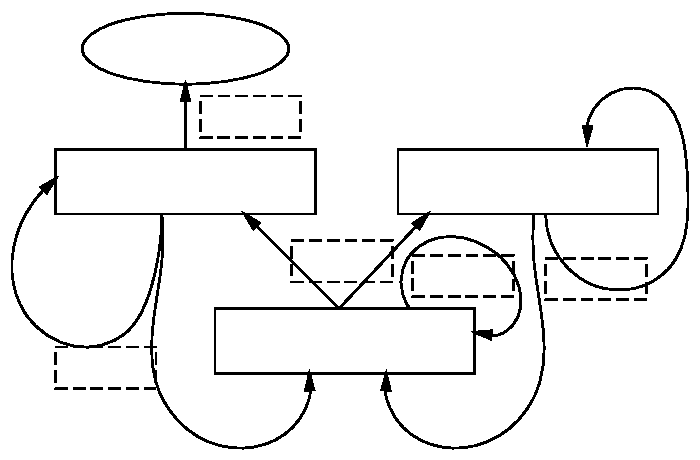
\includegraphics{bull.pdf}}
    \put(218.82,129.60){\fontsize{14.23}{17.07}\selectfont agressive(..)}
    \put(117.56,53.06){\fontsize{14.23}{17.07}\selectfont searchAround(..)}
    \put(145.03,92.94){\fontsize{8.54}{10.24}\selectfont howRed(..)}
    \put(59.92,129.60){\fontsize{14.23}{17.07}\selectfont wander(..)}
    \put(50.59,193.38){\fontsize{14.23}{17.07}\selectfont "GetStacked"}
    \put(201.17,85.86){\fontsize{7.11}{8.54}\selectfont CountDown>0}
    \put(104.39,162.39){\fontsize{8.54}{10.24}\selectfont IRSensor}
    \put(31.64,41.92){\fontsize{7.11}{8.54}\selectfont Random()>0.9}
    \put(266.92,84.44){\fontsize{8.54}{10.24}\selectfont howRed(..)}
    \end{picture}%
  \else
    \setlength{\unitlength}{1bp}%
    \begin{picture}(335.93, 220.08)(0,0)
    \put(0,0){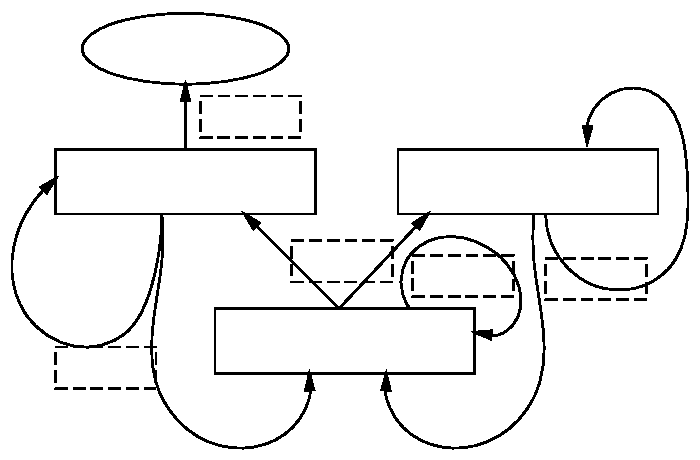
\includegraphics{bull}}
    \put(218.82,129.60){\fontsize{14.23}{17.07}\selectfont agressive(..)}
    \put(117.56,53.06){\fontsize{14.23}{17.07}\selectfont searchAround(..)}
    \put(145.03,92.94){\fontsize{8.54}{10.24}\selectfont howRed(..)}
    \put(59.92,129.60){\fontsize{14.23}{17.07}\selectfont wander(..)}
    \put(50.59,193.38){\fontsize{14.23}{17.07}\selectfont "GetStacked"}
    \put(201.17,85.86){\fontsize{7.11}{8.54}\selectfont CountDown>0}
    \put(104.39,162.39){\fontsize{8.54}{10.24}\selectfont IRSensor}
    \put(31.64,41.92){\fontsize{7.11}{8.54}\selectfont Random()>0.9}
    \put(266.92,84.44){\fontsize{8.54}{10.24}\selectfont howRed(..)}
    \end{picture}%
  \fi
  \caption{\label{pic:bull}%
   Bull behaviour diagram}
  \end{figure}
  
  Aggressive behaviour tries to bump into red obstacles. If it finds out an obstacle not red enough, it
  starts searching again. After four 90 degrees rotations in $searchAround$ are made, 
  the $wander$ behaviour is switched on. From $wander$ state the behaviour 
  can switch back to $searchAround$ or it  ends stacked.
  Let us show how simple the $aggresive$ function can be.

\begin{lstlisting}[language=cs]
double redl = 0.2;
IAsyncResult ar = ada.BeginGetImage(toImg, null, null);
Bitmap a = ada.EndGetImage(ar);
howRed(a, out red, out dir);
if (red > redl) {
  ada.BeginMotors(0.4, 0.4, to, agressive, ada);
} else {
  ar = ada.BeginStop(to, null, null);
  ada.EndFtion(ar);
  ada.BeginGetImage(toImg, searchAround, new CountDown(ada, 3));
}
\end{lstlisting}
  
\subsection{Billiard ball behaviour}\label{billiard}
  The behaviour is invoked by $Billiard$ function. The behaviour is rather simple.
  It goes to a wall and before the wall it stops. Then the robot tries to compute the
  orientation of the wall it turns around to go in a next direction and than it goes straight
  to the next obstacle.
  The behaviour runs without ending until the e-Puck is surrounded by obstacles.

  The $rebound$ function tries to compute the angle of rebound, but as well the simple $go2wall$ function
  implements a restart of the behaviour.
  Let us focus on this part. We will show it on $go2wall$ function in Figure ~\ref{fig:restart}

\begin{figure}[!hbp]
\begin{lstlisting}[language=cs]
static void go2wall(IAsyncResult ar) {
  //value to decide if an obstacle is near enough
  int frontLimit = 1000;  
  //does not throw ElibException
  Epuck ada = (Epuck)ar.AsyncState;
  try {
    // Doesn't create EventWaitHandle because the action has already completed synchronously.
    // Can throw an TimeoutElibException
    int[] ir = ada.EndGetFtion(ar);    
    if (ir[0] + ir[7] > frontLimit)
      ada.BeginStop(to, rebound, ada);
    else {
      //Does not use EndFtion, it saves the EventWaitHandle. We suppose, that it succeeds now or in next rounds.
      ada.BeginMotors(0.2, 0.2, to, null, null);
      // The BeginGetIR command is enqueued in the same momment as BeginMotors, therefor double timeout is used.
      ada.BeginGetIR(2 * to, go2wall, ada);
    }
  } catch (ElibException e) {
    Console.WriteLine("Billiard restarted in go2wall, because of exception:\n" + e.Message);
    // Invokes go2wall function again. It needs to be invoked by BeginGetIR command, because it expects ar with IR values.
    ada.BeginGetIR(to, go2wall, ada);
  }
}
\end{lstlisting}
\caption{\label{fig:restart} } 
\end{figure}

  The exception can be throw on only in call of $EndGetFtion$ at the beginning and 
  no action in the body was done, so the function can be called again from the catch block without problems.

  The problem of this implementation is the logic, not the implementation. 
  The restart of the $go2wall$ function does not solve the problem with 
  slow delivery of IR sensors, it only tries and tries again until enter is pressed.
  The solution will be presented in next behaviours.

  Next interesting feature of this example is not calling the $EndFtion$ to wait until $BeginMotors$ is confirmed.
  We suppose that if the commands of $BeginGetIR$ sensors are delivered, than the $BeginMotors$ are delivered too.
  Furthermore only one command delivered is enough to go to the next obstacle.

\subsection{Exact movement and $GoAndTurn$ behaviour} \label{sec:go}
  Exact movement is a very strong feature of e-Puck. E-Puck uses two stepper motors,
  which allows you to travel exactly 10 cm. The deviation is less than one millimeter.
  E-Puck has also encoders, which allow you to measure the distance of travel with the same resolution.
  On the other hand, communication over Bluetooth brings problems, which are typical for common electric motors.
  Usual motors have an inertia and they do not stop immediately and they do not reach the desired speed at once. The same problem is with 
  {\it Elib} and Bluetooth communication. The commands have a delay.
  A common problem is also with a flat tyre, because one wheel has bigger perimeter than the other.
  Programmers of e-Puck do not have to solve these problems due to good design of e-Puck.

  $GoAndTurn$ is the only behaviour, which does not run in an infinite loop. 
  It just goes around a perimeter of square with side
  of 15 cm. It is based on $goXmiliseconds$ function, which lets the robot ride with given speed for a specified time.
  Functions $TurnAround$ and $goXcm$ are simply built on $goXmiliseconds$. The $square$ function from $GoAndTurn$ behaviour
  simply combines the functions.
  Let us introduce $goXmiliseconds$ function.
\begin{figure}[!hbp]
\begin{lstlisting}
static void goXmiliseconds(Epuck e, double L, double R, int milisec, double addto) {
  int x = e.Working;
  if (x != 0)
    throw new ElibException("It would be extremely inaccurate, if commands are still waiting to be sent.");
  IAsyncResult ar = e.BeginMotors(L, R, addto, null, null);
  AsyncResultNoResult pom = (AsyncResultNoResult)ar;
  pom.Name += "goXms";
  e.EndFtion(ar);
  ar = e.BeginStop(addto, null, null);
  e.EndFtion(ar);
}
\end{lstlisting}
\caption{Function goXmiliseconds} \label{gox}
\end{figure}

  The function needs to have no queued commands in $Epuck$ instance, 
  because it supposes that sending takes almost no time and any waiting makes it very inaccurate.
  The function sends a command to motors, then waits a given time and then stops.
  The idea behind the little heuristic is that every commands sending takes the 
  same time and also the commands transferred to e-Puck and from e-Puck are equally fast.

  More interesting feature presented here is extracting 
  an $AsyncNoResult$ class from $IAsyncResult$ interface. 
  For more information see Section ~\ref{sec:iasync}.
  From user's point of view it is good to know, that $Name$ property can be changed. 
  $Name$ property is used in logging. 
  Its default value is the name of "Begin" function,
  which created the instance of $IAsyncResult$. The $Name$ attribute is a feature of {\it Elib} 
  and is not defined in $IAsyncResult$, therefore the cast is needed for accessing it.

\subsection{Restarting $Go2light$ behaviour}\label{sec:go2light}
  Robot following the light is a typical robotic task. $Go2Light$ behaviour uses only one recursive function, which implements the behaviour.
  The following example also presents a guideline how to cope with unreliable connection 
  in~an~infinite behaviour.

\begin{figure}[!hbp]
\begin{lstlisting}
  
static void recGotoLight(IAsyncResult ar) {
  Epuck ada = (Epuck)ar.AsyncState;
  try {
    ar = ada.BeginGetLight(to, null, null);
    int[] light = ada.EndGetFtion(ar);
    //..omitted part of source code: Debugging printouts
    if (diff_fb > 0) {
      if (light[2] < light[5]) {
        Console.WriteLine("turn around right {0}", diff_lr);
        ar = ada.BeginMotors(speed, 0, to, recGotoLight, ada);
      } else {
      //..omitted part of source code: the lighst is on front left, back right,...
      }
    }
    //there is no need to repeat EndFtion in the branches
    ada.EndFtion(ar);
  } catch (TimeoutElibException) {
    exceptionOccured_Restart(ada);
  }
}
\end{lstlisting}
\caption{Function $recGotoLight$ function} \label{go2light}
\end{figure}
  See the~clear structure of $recGotoLight$ function is in source code in Behaviours.cs file. 
  Let us explore the interesting $exceptionOccured\_Restart$ function in Figure \ref{restart}.
  The function ends the session with real e-Puck and closes a serial port by calling $Dispose$ method.
  After the disposal, the commands can not be sent to e-Puck and we have to create a new connection. We use the same parameters.
  Optionally, here is the place to ask the user of behaviour to change a port name.
  The same approacapproachh is used in $KofGoXcm$, which will be presented below.
\begin{figure}[!hbp]
\begin{lstlisting}
static void exceptionOccured_Restart(Epuck ada) {
  //Reconnect again to e-Puck
  ada.Dispose();
  ada = new Epuck(ada.Port, ada.Name);
  restarts--;
  if (restarts >= 0) {
    Console.WriteLine("Remaining " + restarts.ToString() + " restart(s). Press enter to continue");
    ada.BeginStop(to, recGotoLight, ada);
  } else {
    Console.WriteLine("End of Go2Light, because all " + restarts_startingValue.ToString() + "restarts have been used.");
    Console.WriteLine("Behaviour has finished. Press enter to perform next actions");
  }
}
\end{lstlisting}
\caption{Function $exceptionOccured\_Restart$ function} \label{restart}
\end{figure}

\subsection{Behaviour with return implemented via $Epuck's$ basic interface}\label{sec:kofgoxcm}
  The behaviour is invoked by $KofGoXcm$ function. 
  The robot goes specified amount of centimeters. 
  If the connection breaks during the behaviour, 
  the behaviour ask the user to repair the connection and to keep e-Puck running. 
  If the connection is repaired successfully then e-Puck goes to the destination, 
  where it should have ended before the connection failure.

  The behaviour  uses $Epuck's$ basic interface,	
  which has been introduced in Section ~\ref{sec:touching}.
  It has some design consequences. The example has two implementations, in fact two behaviours. 
  The behaviour, which has a good connection at disposal,
  and the behaviour, which has to deal with a broken connection.
  We also keep the guideline from Section ~\ref{safedis}. 
  It says, that the asynchronous call should be made only once at the end of a function.
  It is necessary to avoid parallelism and problems with ending of the behaviour.

  In summary, the amount of functions grows rapidly, 
  because we can not easily synchronously wait to answers from e-Puck
  and furthermore we have to implement two kinds of functions: $Kof$ and $Okf$ callbacks.
  The implementation of $okf(..)$ callbacks is straightforward. 
  We will focus on a function, which is called to stop the e-Puck after it travelled the required distance.

  Let us remind of the $Epuck$ basic interface.
  In Figure ~\ref{stopKof} class $RobotAndTime$ is used. 
  As you can see, the structure of the code does not differ from $IAsyncResul$. 
  First the necessary cast is performed in order to 
  extract $RobotAndTime$ class, then the logic is implemented and in the end 
  the commands to e-Puck are sent.
  The $Kof$ and $Okf$ commands use the same state argument for passing data,
  e.g. $RobotAndTime$ instance. The state argument together 
  with timeout are obligatory and are located at the end of functions.
  The $Okf$ callback for a sensor command has additional first argument. 
  The first argument is used to return sensor values. For example
  the callback for $GetIR$ command looks like $void\ OkGetIR(int[]\ values,\ object\ state);$.
  
\begin{figure}[!hbp]
\begin{lstlisting}
static void stopKof(object robotAndTime) {
  Console.WriteLine("stopKof was called.");
  RobotAndTime x = (RobotAndTime)robotAndTime;
  x.stopKof++;
  if (x.stopKof > 5) {
    if (!reconnect(x))
      return;
    else
      x.stopKof = 0;
  }
  double time = Stamp.Get() - x.StartTime;
  if (travelled(time, x.Speed) < (x.Cm + 0.05))
    x.E.Stop(stopOkf, stopKof, x, to);
  else {
    Console.WriteLine("We missed the destination spot, we return back, try to repair the connection.");
    x.Cm = travelled(x.StartTime, x.Speed) - x.Cm;
    x.Speed = -x.Speed;
    x.StartTime = Stamp.Get();
    x.E.Motors(x.Speed, x.Speed, goOkf, goKof, x, to);
  }
}

class RobotAndTime {
  // Lot of parts omitted!! 
  // The thread.Safe read and write are missing!!
  public double StartTime;
  double cm;
  double speed;
  public volatile int stopKof = 0;
  public volatile int goKof = 0;
}
\end{lstlisting}
\caption{$Kof$ callback $stopKof$} \label{stopKof}
\end{figure}
  The logic of this example is very interesting. After five unsuccessful attempts to stop,
  the $reconnect$ function prompts the user to repair the connection. 
  If the user refuse to continue, no other function is invoked, and the behaviour is ended.
  Otherwise, the actions for going to the desired place are executed.
  If the robot does not drive away too far, the $Stop$ function is called again.
  The $Stop$ function calls $stopKof$ function as its $Kof$ callback.
  If the robot travels too long then it has to go in the opposite direction.
  The change of the direction is done in the second branch of the $if$ command.

  %\input{kofgoxcm.TpX}
  \begin{figure}[!hbp]
  \centering
  \setlength{\unitlength}{1bp}%
  \begin{picture}(289.13, 262.60)(0,0)
  \ifpdf
    \put(0,0){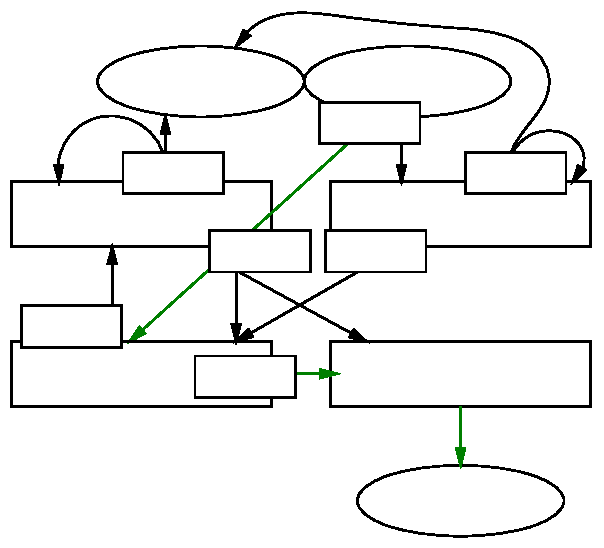
\includegraphics{kofgoxcm.pdf}}
  \else
    \setlength{\unitlength}{1bp}%
  \fi
  \put(0,0){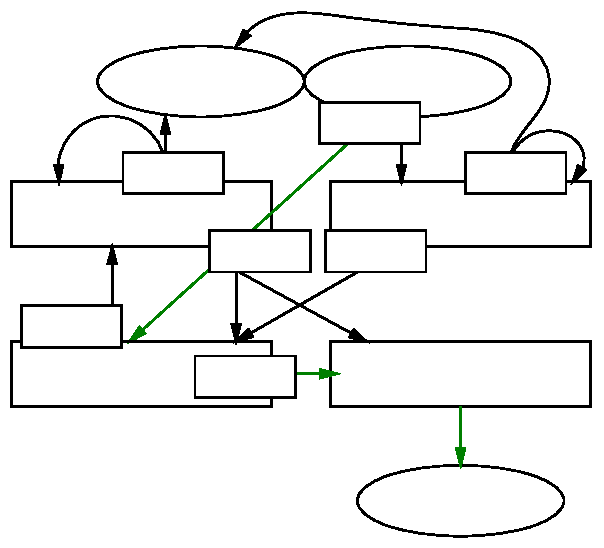
\includegraphics{kofgoxcm}}
  \put(194.73,156.13){\fontsize{14.23}{17.07}\selectfont goKof(..)}
  \put(36.94,156.13){\fontsize{14.23}{17.07}\selectfont stopKof(..)}
  \put(157.14,219.91){\fontsize{14.23}{17.07}\selectfont KofGoXcm(..)}
  \put(57.93,219.91){\fontsize{14.23}{17.07}\selectfont User stop it!}
  \put(190.01,79.60){\fontsize{14.23}{17.07}\selectfont stopOkf(..)}
  \put(178.02,18.65){\fontsize{14.23}{17.07}\selectfont We succeeded!}
  \put(41.66,79.60){\fontsize{14.23}{17.07}\selectfont goOkf(..)}
  \put(11.42,103.88){\fontsize{7.11}{8.54}\selectfont Motors(ok,ko)}
  \put(103.11,140.03){\fontsize{7.68}{9.22}\selectfont Stop(ok,ko)}
  \put(157.41,140.03){\fontsize{7.11}{8.44}\selectfont Motors(ok,ko)}
  \put(96.03,79.79){\fontsize{7.68}{9.22}\selectfont Stop(ok,ko)}
  \put(65.30,177.58){\fontsize{7.68}{9.22}\selectfont Reconnect?}
  \put(229.71,177.58){\fontsize{7.68}{9.22}\selectfont Reconnect?}
  \put(154.57,201.68){\fontsize{7.11}{8.44}\selectfont Motors(ok,ko)}
  \end{picture}%
  \caption{\label{pic:kofgoxcm}%
   $KofGoXcm$ basic $Epuck's$ interface implementation}
  \end{figure}

%%todo processing the image 
\subsection{Logging of $Epuck$ actions and image processing}\label{sec:logging}
  In the file $TipsAndTricks.cs$ there is located a simple example of image processing 
  of a picture from e-Puck's camera.
  The example is invoked by the function $ShowProcessedImage$ and it displays a window, 
  where a black and white image is processed.
  The white is instead of red colour and black represents the other colours. 
  A nice test of this function is to place
  the e-Puck's box with the e-Puck logo in front of the camera. 

  The function $LoggingExample$ uses the function $ConsoleTestSensorsTimeout$, 
  which has been presented at the beginning of this section in ~\ref{sec:touching}.
  It runs the function twice, each time with different timeout. 
  The logging to file specified in $name$ property is turned on.
  Try to run the function. 
  Let us see the body of the function.
\begin{lstlisting}
ada.LogStream = new StreamWriter(new FileStream(name, FileMode.OpenOrCreate, FileAccess.Write));
ada.StartLogging();
for (i = 0; i < 2; ++i) {
  double to=1.0 / (i + 1);
  ada.WriteToLogStream("ConsoleTestSensors with timeout :"+to.ToString());
  ConsoleTestSensorsTimeout(ada, to);
}
ada.StopLogging();
\end{lstlisting}
  Logging to a file is really simple. In needs only stream, where the log is written. 
  After the start of logging all actions that send commands to e-Puck, performed on $ada$ instance of $Epuck$ are logged
  to file on path $name$.
  $WriteToLogStream$ method inserts a commented line to the log file.

\section{Elib tools (et)}\label{sec:et}
  {\it Elib} offers a standalone command line application, which
  parses the log from {\it Elib}. It is meant to be the base tool for a programmer,
  who wants to statistically analyse a log from $Epuck$ class.

  Et can be used only from the command line and parses the log row by row.
  It reads the log file, performs a chosen action and writes the result to the output file.
  If user does not specify the file it writes or read from, respectively, to command line.
  Elib tools supports three operation. Two of them process numeric data.
  The first operation counts an average of a selected column from a log file.
  The next operation sorts out rows, which have in specified column values from a given range.
  The last implemented operation separates rows, 
  which have in specified column a value from a given collection of words.
  Elib tools application skips the rows beginning with $'\#'$, 
  which is in {\it Elib} by default a comment in the log file.
  Let us look at the usage. The most important command is the second row, which invokes the help file.
  The help file introduces a complete usage of et command.
  Let us remark, that this invocation was performed in PowerShell on Windows. On Linux you need to add "mono" before every program,
  which was compiled for .Net or Mono.
\begin{verbatim}
>>et -s sourcelog.txt -d output.txt Avg 0
>>et -h
et (Elib Tools) HELP FILE
...here the help file continues
\end{verbatim}

\subsection*{Design of {\it Elib Tools}}\label{sec:design}
  The purpose of {\it Elib Tools} is to be a simple tool for parsing a log file from {\it Elib}.
  The application is written in order to be as robust as possible.
  Wrong arguments do not throw any exception, but the application does no action.

  The main contribution of {\it Elib Tools} application is its design, which can be easily extended.
  The application can be easily changed according to specific needs of a programmer.
  The programmer needs to modify $parseArguments$ argument function.
  As you can see, the $parseArguments$ function returns only paths 
  of the source and the destination file and $Action$ object.
\begin{lstlisting}
Action action = parseArguments(args, out source, out destination);
\end{lstlisting}
  
  $Action$ object is an abstract class, which is introduced below in this section. It provides
  an interface for performing operation on every row of the source file.
  If a new functionality is added, it could be implemented only by deriving 
  a class from $Action$ and by overriding
  two functions. Let us describe an example of Avg command. Lets look first at $Action$ class.
\begin{figure}[!hbp]
\begin{lstlisting}
abstract class Action {
  const string Comment = "#";
  protected int column;
  protected TextReader r;
  public TextReader R { get { return r; } set { r = value; } }
  protected TextWriter w;
  public TextWriter W { get { return w; } set { w = value; } }
  protected char[] sep;
  public char[] Separators { get { return sep; } set { sep = value; } }
  public Action(int Column) {
    column = Column;
  }
  public void DoAction() {
    string line = null;
    while ((line = r.ReadLine()) != null) {
      if (!line.StartsWith(Comment))
        LineAction(line);
    }
    LastAction();
  }
  protected virtual void LastAction() { /*usually does nothing and is called after all lines are processed*/}
  protected abstract void LineAction(string line);
}
\end{lstlisting}
\caption{$Action$ abstract class for performing row operation}\label{action}
\end{figure}

  The $Average$ class, which inherits from $Action$ class, computes 
  the average by calling a method $DoAction()$ inherited from $Action$ class. 

\begin{figure}[!hbp]
\begin{lstlisting}
class Average : Action {
  long count;
  double avg;
  public Average(int Column)
  : base(Column) {
    count = 0;
    avg = 0;
  }
  protected override void LineAction(string line) {
    count++;
    avg *= (count - 1) / (double)count;
    try {
      avg += (Double.Parse((line.Split(sep)[column])) / count);
    } catch (FormatException e) {
      Console.WriteLine("Avg has to be done from Integer. Error: " + e.Message);
      avg = double.NaN;
    }
    }
    protected override void LastAction() {
    w.WriteLine("{0:F8}", avg);
  }
}
\end{lstlisting}
\caption{$Average$ class}\label{average}
\end{figure}

%  $Average$ class computes average step by step in order to avoid 
%  overflow of a variable in parsing large log files. The overflow
%  of a variable is postponed by computing average in every step from the previous average
%  and the new value, 
%  because the typical implementation by sum all the values and after then diving it 
%  with its amount leads to overflow of the sum much more quickly.

\section{Purpose of {\it Elib} and its properties}
  In this chapter we have presented {\it Elib} and the guidelines, 
  which are convenient to follow using {\it Elib}. 
  This section follows up to contents of the previous sections and introduces a view from,
  which was the {\it Elib} created.

  {\it Elib} library was designed in order to help students of mobile robotics	
  with controlling e-Puck by their programs.
  {\it Elib} extends possibilities of e-Puck processor, 
  which can perform a very limited range of algorithms
  due too its low performance.
  Moreover {\it Elib} provides a user with numerous examples. The examples are commented
  and can be easily modified.
  On the other hand, a program, which use {\it Elib}, gives up of direct control over robot,
  which can be observed the best on $GoAndTurn$ behaviour in Section ~\ref{sec:go}.

  We have presented a few of simple behaviours, which control e-Puck, 
  but much more can be done with {\it Elib}.
  {\it Elib} can be used easily for controlling more than one e-Puck at the same time
  by creating more sessions using
  different instances of $Epuck$ class. Programs, which need more than 8 KB of memory on e-Puck such 
  as genetic programs or neural networks, can easily control e-Puck over Bluetooth.

  The real challenge is processing a picture from e-Puck, 
  because the dsPic processor of e-Puck is not sufficient
  and also {\it Elib} needs to wait quite a lot of time for a picture.
  On the other hand, $Bull$ behaviour successfully use the camera to grab the picture
  and also a graphical application {\it Elib Joystick} shoots the pictures with the camera.

  {\it Elib Joystick} is a graphical application, which makes all sensors and actuators of e-Puck accessible in one window.
  It also supports capturing of an image, which is presented enlarged to the user.
  The graphical application runs in Single Thread Apartment on Windows, which means that the controls of the window can 
  be accessed only from the main thread.
  In order to update the sensors {\it Elib Joystick} use either $EndFtion$ or a $Dispatcher$.
  $Dispatcher$ is a class, which allows to access the controls from a different thread. 
  It is specific according to the technology,
  which is used to run the graphical part of the application. 
  {\it Elib Joystick} uses Windows Presentation Foundation and
  uses a dispatcher to capturing image. The other operation, 
  which has timeout 0.1 s, accesses the controls synchronously using
  either $EndFtion$ or $EndGetFtion$. See Section ~\ref{sec:bull} for information 
  about these functions. {\it Elib Joystick} is introduced in appendix ~\ref{app:joystick}.

  {\it Elib} can access all sensors of e-Puck. See the Chapter ~\ref{sec:epuck} 
  for more information about e-Puck's sensors and actuators.
  However, the camera is not used in the full resolution,
  because the e-Puck processor has no place to store the captured image.
  The {\it Elib} captures only the amplitude of sounds from e-Pucks microphones,
  because {\it ELib} library depends on {\it BTCom}.
  The frequency of a sound can be computed on e-Puck
  using Fast Fourier Transformation on e-Puck, 
  but the {\it BTCom} does not implement it.

  To conclude, {\it Elib} offers almost all sensors of e-Puck in full quality. 
  It also controls all of e-Puck's actuators.
  Furthermore, it offers much more comfort than a programming e-Puck's processor directly. 
  Read Section \ref{sec:design} about the advantages
  of remote control. 
  Last but least, {\it Elib} can be used from all .Net languages 
  including $C\#$, $Visual Basic$, $F\#$,
  which is a functional language of .Net based OCaml,
  or $Iron Python$, which is a .Net implementation of Python. On Mono runtime, 
  which runs both on Linux and Windows, the $C\#$ language can be used.
  The {\it Elib} is compatible with .Net 2.0 \cite{net} and higher 
  and with Mono \cite{mono} 2.0 and higher.

